\section{Linear Maps}

	\begin{definition}[Linear Map]
		Given vector spaces $V, W$ over some field $\mathbb{F}$, a \textbf{linear map} is a function 
		\begin{equation}
		  T: V \to W
		\end{equation}
		satisfying $T(au + bv) = a T(u) + b T(v)$. 
	\end{definition}

  Linear maps over vector spaces over different fields are generally not well defined since the definition of homomorphisms do not cover the fields in which vector spaces are associated with. 

	\begin{example}[Linear Map from $\mathbb{R}^2$ to $\mathbb{R}^2$]
		A nice visual is to imagine a linear map as ``mapping squares to parallelograms.''

		\begin{figure}[H]
			\centering 
			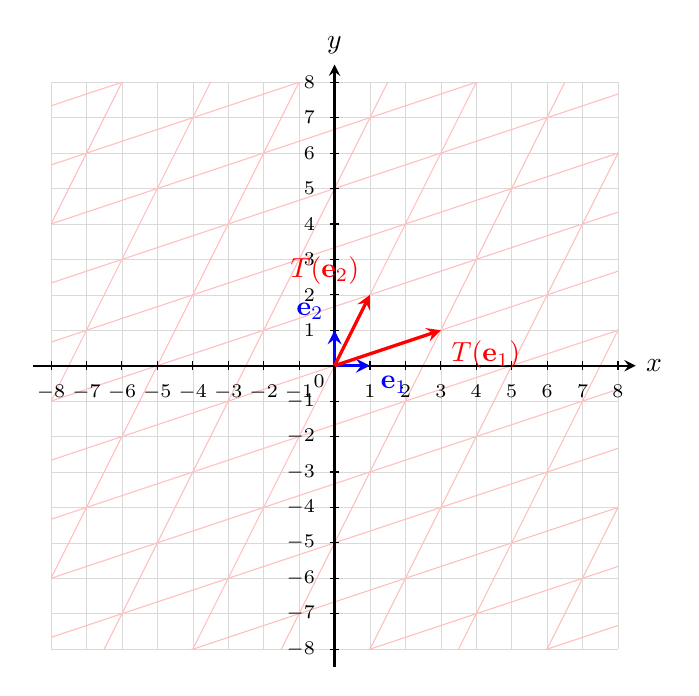
\begin{tikzpicture}[scale=0.45, >=stealth]
				% Plot window
				\def\xmin{-8}
				\def\xmax{8}
				\def\ymin{-8}
				\def\ymax{8}

				% Original grid
				\draw[step=1, gray!30, very thin] (\xmin,\ymin) grid (\xmax,\ymax);

				% Image of the grid under T
				% T(e_1) = (3,1), T(e_2) = (1,2)
				% So T(x,y) = x(3,1) + y(1,2) = (3x+y, x+2y)
				\begin{scope}
					\clip (\xmin,\ymin) rectangle (\xmax,\ymax);

					% Images of vertical grid lines x = k
					\foreach \k in {-8,-7,...,8} {
						\draw[red!25, thin]
							({3*\k + (-8)}, {\k + 2*(-8)})
							--
							({3*\k + 8}, {\k + 2*8});
					}

					% Images of horizontal grid lines y = k
					\foreach \k in {-8,-7,...,8} {
						\draw[red!25, thin]
							({3*(-8) + \k}, {(-8) + 2*\k})
							--
							({3*8 + \k}, {8 + 2*\k});
					}
				\end{scope}

				% Original axes
				\draw[->, thick] (-8.5,0) -- (8.5,0) node[right] {$x$};
				\draw[->, thick] (0,-8.5) -- (0,8.5) node[above] {$y$};

				% Tick marks and labels
				\foreach \x in {-8,-7,...,-1,1,2,...,8} {
					\draw (\x,0.12) -- (\x,-0.12)
						node[below=2pt] {\scriptsize $\x$};
				}

				\foreach \y in {-8,-7,...,-1,1,2,...,8} {
					\draw (0.12,\y) -- (-0.12,\y)
						node[left=2pt] {\scriptsize $\y$};
				}

				% Origin
				\node[below left] at (0,0) {\scriptsize $0$};

				% Original basis vectors
				\draw[->, blue, very thick] (0,0) -- (1,0)
					node[below right] {$\mathbf e_1$};

				\draw[->, blue, very thick] (0,0) -- (0,1)
					node[above left] {$\mathbf e_2$};

				% Images of the basis vectors
				\draw[->, red, very thick] (0,0) -- (3,1)
					node[below right] {$T(\mathbf e_1)$};

				\draw[->, red, very thick] (0,0) -- (1,2)
					node[above left] {$T(\mathbf e_2)$};
			\end{tikzpicture}
			\caption{The basis vector $(1, 0)$ gets mapped to $(3, 1)$, and the vector $(0, 1)$ gets mapped to $(1, 2)$. Due to linearity, the map is completely determined. Given any $v \in \mathbb{R}^2$, since $\{e_1, e_2\}$ spans the domain, we can write $v = a_1 e_1 + a_2 e_2$. Therefore, $T(v) = T(a_1 e_1 + a_2 e_2) = a_1 T(e_1) + a_2 T(e_2)$. This means that we just need to take the same linear combination of the images of the basis vectors to find the image of $v$.} 
			\label{fig:linear_map_visual}
		\end{figure}
	\end{example}

	\begin{example}[Left Matrix Multiplication]
		Left matrix multiplication is a linear map from $\mathbb{R}^2$ to $\mathbb{R}^2$. Consider the matrix 
		\begin{equation}
			A = \begin{pmatrix} 3 & 1 \\ 1 & 2 \end{pmatrix}
		\end{equation} 
		Therefore 
		\begin{align}
			A(av + bw) & = \begin{pmatrix}
				3(a v_1 + b w_1) + (a v_2 + b w_2) \\
				(a v_1 + b w_1) + 2(a v_2 + b w_2)
			\end{pmatrix} \\ 
								 & = a \begin{pmatrix} 
				3v_1 + v_2 \\ 
				v_1 + 2 v_2 
			\end{pmatrix} + b \begin{pmatrix} 
				3w_1 + w_2 \\ 
				w_1 + 2w_2 
			\end{pmatrix} \\ 
								 & = a \begin{pmatrix} 3 & 1 \\ 1 & 2 \end{pmatrix} \begin{pmatrix} v_1 \\ v_2 \end{pmatrix} + b \begin{pmatrix} 3 & 1 \\ 1 & 2 \end{pmatrix} \begin{pmatrix} w_1 \\ w _2 \end{pmatrix} = a A v + a Bw
		\end{align}
	\end{example}

	\begin{example}[Differentiation]
		Let $C^1 [a, b]$ be the vector space of all continuously differentiable functions $f: [a, b] \to \mathbb{R}$. Then, recall that 
		\begin{align}
			\frac{d}{dx} (f + g) & = \frac{d}{dx} f + \frac{d}{dx} g \\ 
			\frac{d}{dx} (cf) & = c \bigg( \frac{d}{dx} f \bigg)
		\end{align}
		Therefore, this makes differentiation a linear operator. 
	\end{example}

	\begin{example}[Integration]
		Let $C^0 [a, b]$ be the vector space of all continuous functions $f: [a, b] \to \mathbb{R}$. Then, recall that 
		\begin{align}
			\int_a^b (f + g) & = \int_a^b f + \int_a^b g \\ 
			\int_a^b cf & = c \int_a^b f
		\end{align}
		Therefore, this makes integration a linear operator. 
	\end{example}

\subsection{Image and Null Space}

  Let's first recall some of the basic properties an notation for functions. 

  \begin{definition}[Image]
    The \textbf{image} of linear map $T: U \to V$, denoted $\im(T)$, is the range of $T$. 
    \begin{equation}
      \im(T) \coloneqq \{T(u) \in V \mid u \in U\}
    \end{equation}
    We claim $\im(T)$ is a subspace of $V$. 
  \end{definition}
  \begin{proof}
    It suffices to show that the image is a subspace. 
  \end{proof}

  \begin{definition}[Rank]
    The \textbf{rank} of a linear map $A$ is the dimension of its image. 
  \end{definition}

  \begin{definition}[Nullspace, Kernel]
    The \textbf{nullspace} of $T: U \to V$, denoted $\mathrm{ker}(T)$, is the 
    is the kernel of $T$. 
    \begin{equation}
      \mathrm{ker}(T) \coloneqq \{ u \in U \mid T(u) = 0\}
    \end{equation}
    We claim $\mathrm{ker}(T)$ is a subspace of $U$. 
  \end{definition}
  \begin{proof}
    It suffices to show that the image is a subspace. 
  \end{proof}

	\begin{example}[Image and Kernel of Quotient Map]
    Let $U_1$ be a subspace of $U$ and given the quotient map
    \begin{equation}
      \pi: U \longrightarrow U / U_1
    \end{equation}
    Then, 
    \begin{equation}
      \text{ker}\,\pi = U_1, \; \im{\pi} = U / U_1
    \end{equation}
    Note that a quotient map is always surjective. 
  \end{example} 
	
	A key problem in linear algebra is to solve the following equation $Ax = b$, i.e. what is the set of all $x$'s such that $Ax = b$? The following theorem reduces this problem to finding one solution and the kernel of $A$. 

	\begin{theorem}[]
    Given linear map $A: V \longrightarrow U$ and $b \in U$, then all solutions to the equation $Ax = b$ is of the form 
		\begin{equation}
			a + \ker(A) \coloneqq \{a + v \in V \colon v \in \ker(A)\}
		\end{equation}
		where $a$ is one solution. 
  \end{theorem}
	\begin{proof}
		Let $a, a^\prime$ be any two solutions. Then, $Aa = b$ and $A a^\prime = b$. So 
		\begin{equation}
		  A a - A a^\prime = 0 \implies A(a - a^\prime) = 0 \implies a - a^\prime \in \ker(A)
		\end{equation}
	\end{proof}

  \begin{corollary}
    A linear map $A$ is injective if and only if $\ker A = 0$.
  \end{corollary}

  \begin{theorem}[Rank Nullity Theorem]
    Let $T: U \longrightarrow V$ be linear. Then, 
    \begin{equation}
      \dim \ker T + \dim \im T = \dim U
    \end{equation}
    This theorem is quite intuitive, if we visualize the map. 

    \begin{figure}[H]
      \centering 
      \begin{tikzpicture}
        % Add R³ label for the left side
        \node at (-2.9,2.1) {$\mathbb{R}^3$};
        
        % Add R² label for the right side
        \node at (2,2.1) {$\mathbb{R}^2$};
        
        % Left diagram - Parallelogram with kernel
        \begin{scope}[shift={(-4,0)}]
          % Rotate the entire picture 30 degrees clockwise
          \begin{scope}[rotate=-30]
            % Define coordinates for the parallelogram
            \coordinate (A) at (-2,-1);
            \coordinate (B) at (2,-1);
            \coordinate (C) at (1,1);
            \coordinate (D) at (-3,1);
            
            % Draw the parallelogram with red fill
            \fill[red, opacity=0.3] (A) -- (B) -- (C) -- (D) -- cycle;
            \draw (A) -- (B) -- (C) -- (D) -- cycle;
            
            % Draw the dashed portion where the line intersects the parallelogram in blue
            \draw[dashed, thick, blue] (-0.5,-2) -- (-0.5,2);
            
            % Add a dot at intersection point
            \filldraw (-0.5,0) circle (2pt);
            
            % Label the dashed line in blue
            \node[blue] at (0.8,0) {$\mathrm{ker}(T)$};
          \end{scope}
        \end{scope}
        
        % Arrow connecting the two diagrams
        \draw[-{Stealth[length=3mm,width=2mm]}] (-1,0) -- (1,0);
        \node at (0,0.5) {$T$};
        
        % Right diagram - Real plane
        \begin{scope}[shift={(4,0)}]
          % Fill the background with red
          \fill[red, opacity=0.3] (-2.5,-2.5) rectangle (2.5,2.5);
          
          % Draw the x and y axes
          \draw[->] (-2.2,0) -- (2.2,0) node[right] {$x$};
          \draw[->] (0,-2.2) -- (0,2.2) node[above] {$y$};
          
          % Add tick marks
          \foreach \x in {-2,-1,1,2}
            \draw (\x,0.1) -- (\x,-0.1) node[below] {$\x$};
          \foreach \y in {-2,-1,1,2}
            \draw (0.1,\y) -- (-0.1,\y) node[left] {$\y$};
          
          % Mark the origin with a blue point
          \filldraw[blue] (0,0) circle (2.5pt);
        \end{scope}
      \end{tikzpicture}
      \caption{We just have to realize that given a linear transformation mapping from a $n$-dimensional $V$ to a $m$-dimensional $U$, every vector in $V$ will either get mapped to $0 \in U$ or will get mapped to a nonzero vector in $U$. In this case, the kernel will get mapped to $0$ and everything else is (not always, but in this case) $\mathbb{R}^2$. } 
      \label{fig:rank_nullity}
    \end{figure}
  \end{theorem}
  \begin{proof}
    
  \end{proof}

\subsection{Invertibility} 

  We now introduce the concepts of left and right invertibility of linear mappings. 

  \begin{theorem}[Left/Right-Invertibility]
    A linear mapping $T: U \longrightarrow V$, with $\dim{U} = n, \dim{V} = m$, is \textbf{left-invertible}. That is, there exists linear $S$ such that 
    \begin{equation}
      S T = I
    \end{equation}
    if and only if $T$ is injective $\iff$ rank$(T) = n$. Linear $T$ is \textbf{right-invertible}, that is, there exists linear $S$ such that 
    \begin{equation}
      T S = I
    \end{equation}
    if and only if $T$ is surjective $\iff$ rank$(T) = m$. 
  \end{theorem}
  \begin{proof}
    We will only prove the case for left-invertibility. Right invertibility follows analogously. 
    \begin{enumerate}
      \item $(\leftarrow)$ $T$ is injective $\implies$ rank$(T) = \dim{U} = \dim{\im{T}}$. Let $(\im{T})^\prime$ exist such that 
      \begin{equation}
        \im{T} \oplus (\im{T})^\prime = V
      \end{equation}
      We define the isomorphism 
      \begin{equation}
        \Tilde{T}: V \longrightarrow \im{T}
      \end{equation}
      and then define $S$. Given that $v = w + w^\prime \in V$, with $w \in \im{T}, w^\prime \in (\im{T})^\prime$, 
      \begin{equation}
        S : V \longrightarrow U, \; S(v) \equiv \Tilde{T}^{-1} (v)
      \end{equation}
      $\implies S T (u) = \Tilde{T}^{-1} T (u) = u \iff S T = I$. 

      \item $(\rightarrow)$ We prove the contrapositive. $T$ is not injective $\implies \dim{\ker{T}} > 0 \implies $ there exists 2 linearly independent vectors $x, y \in U$ such that
      \begin{equation}
        T x = T y
      \end{equation}
      Assume that a left inverse $S$ exists. Then 
      \begin{equation}
        x = S T x = S T y = y \implies x = y
      \end{equation}
      leading to a contradiction $\implies$ the left-inverse does not exist. 
    \end{enumerate}
  \end{proof}

  \begin{definition}[Inverse]
    The inverse of a linear map $A$, denoted $A^{-1}$ is a unique linear map satisfying 
    \begin{equation}
      A A^{-1} = A^{-1} A = I
    \end{equation}
    where $I$ is the identity map. 
  \end{definition}

  \begin{corollary}
    A linear map is invertible if and only if it is an isomorphism. 
  \end{corollary} 

\subsection{Sets of Linear Maps}

	We have linear maps, but what can we do with multiple linear maps? It turns out that the set of all linear maps from $V$ to $W$ is itself a vector space! 

	\begin{theorem}[Vector Space of Linear Maps]
	  Let $V, W$ be vector spaces. Then, the set of all linear maps $T: V \to W$, denoted $\mathcal{L}(V, W)$, is a vector space. That is given linear maps $T, S: V \to W$ and scalars $a, b \in \mathbb{F}$, the map $aT + bS: V \to W$ is also linear. 
	\end{theorem}
	\begin{proof}
		We prove linearity of $T + S$ first. Given $u, v \in V$, $c \in \mathbb{F}$, 
		\begin{align}
			(T + S)(u + v) & = T(u + v) + S(u + v) = T(u) + T(v) + S(u) + S(v) = (T + S)(u) + (T + S)(v) \\ 
			(T + S)(cu) & = T(cu) + S(cu) = c T(u) + c S(u) = c \big(T(u) + S(u)\big) = c (T + S)(u)
		\end{align}
		To prove linearity of $aT$, we have 
		\begin{align}
			(aT)(u + v) & = a T(u + v) = a \big( T(u) + T(v) \big) = a T(u) + a T(v) = (aT)(u) + (aT)(v) \\ 
			(aT)(cu) & = a T(cu) = ac T(u) = ca T(u) = c(aT)(u)
		\end{align}
	\end{proof}

	If we restrict it to be the set of all endomorphisms, it turns out to be a bit more than that, since we can also compose mappings. 

	\begin{lemma}[Composition of Linear Maps is Linear]
	  Given linear maps $T: U \to V$ and $S: V \to W$, the composition $S \circ T$---denoted $ST$---is a linear map. 
	\end{lemma}
	\begin{proof}
		We see that for addition, given $v, w \in V$, 
		\begin{equation}
			(ST)(v + w)  = S(T(v) + T(w)) = S(T(v)) + S(T(w)) = (ST)(v) + (ST)(w)
		\end{equation}
		For scalar multiplication, given $c \in \mathbb{F}$, $v \in V$, 
		\begin{equation}
			(ST)(cv) = S(T(cv)) = S(c T(v)) = c S(T(v)) = c (ST)(v)
		\end{equation}
	\end{proof}

  In the theorem above, it seems like composition acts sort of like multiplication. Recall that such an algebraic structure that has both the properties of a vector space and multiplication is called an \hyperref[alg-def:algebra]{algebra}. 

	\begin{theorem}[Algebra of Linear Maps]
	  Let $V$ be a vector space. Then, the set of all linear maps $T: V \to V$, denoted $\mathcal{L}(V)$, is a noncommmutative associative algebra. 
	\end{theorem}
	\begin{proof}
		We prove the axioms of an algebra. 
		\begin{enumerate}
		  \item \textit{Distributive Property}. Composition is (right and left) distributive with respect to addition. 
			\begin{align}
				(R + S) \circ T & =  R \circ T + S \circ T \\
				T \circ (R + S) & =  T \circ R + T \circ S 
			\end{align}
		\end{enumerate}
	\end{proof}

	Since $\mathcal{L}(V)$ is a vector space, we can endow it with a norm itself. 

  \begin{definition}[Operator Norm]
		Let $V, W$ be normed vector spaces. Given linear map $A \in \mathcal{L}(V, W)$, the \textbf{operator norm} is defined as the norm
		\begin{equation}
			\|A\| \coloneqq \sup_{\|v\| = 1} \|Av\|
		\end{equation}
  \end{definition} 
	\begin{proof}
	  We prove the 3 properties of the norm. 
		\begin{enumerate}
			\item \textit{Positive Definiteness}. Given linear map $A \in \mathcal{L}(V, W)$, $\|Av\| \geq 0 \implies \|A\| \geq 0$. Also, $\|A\| = 0$ iff $\|Av\| = 0$ for all unit $v \in V$ iff $A = 0$. 

			\item \textit{Absolute Homogeneity}. Given linear map $A \in \mathcal{L}(V, W)$ and $c \in \mathbb{F}$, 
				\begin{equation}
					\|cA\| = \sup_{\|v\| = 1} \|(cA)v\| = \sup_{\|v\| = 1} |c| \|Av\| = |c| \sup_{\|v\| = 1} \|Av\| = |c| \|A\|
				\end{equation}

			\item \textit{Triangle Inequality}. Given linear maps $A, B \in \mathcal{L}(V, W)$, 
				\begin{equation}
					\|A + B\| \coloneqq \sup_{\|v\| = 1} \|(A + B) v\| = \sup_{\|v\| = 1} \|Av\| + \|Bv\| \leq \sup_{\|v\| = 1} \|Av\| + \sup_{\|v\| = 1} \|Bv\| = \|A\| + \|B\|
				\end{equation}
		\end{enumerate}
	\end{proof}

	Note that the operator norm is not an instrinstic property of the linear map. It depends on the norms endowed on the domain and codomain! There is another norm called the Frobenius norm, but this requires a basis. 

	\begin{lemma}[Operator Norm Bound]
		\label{thm:operator_norm_bound}
		Let $V, W$ be normed vector spaces. For any linear map $A: V \to W$ and $v \in V$, 
		\begin{equation}
		  \|Av\| \leq \|A\| \|v\|
		\end{equation}
	\end{lemma}
	\begin{proof}
	  Immediate by definition.
	\end{proof}

	\begin{lemma}[Uniform Continuity of Linear Maps]
		Let $V, W$ be finite-dimensional normed vector spaces. For all $A \in \mathcal{L}(V, W)$, $\|A\| < +\infty$ and $A: V \to W$ is uniformly continuous over $V$. 
	\end{lemma}
	\begin{proof}
		Since all norms on finite-dimensional vector spaces are equivalent, let us choose the $L_2$ norm. Let $v_1, \ldots, v_n$ be a basis for $V$. Then, for any unit $v \in V$, we can expand it as $v = c_1 v_1 + \ldots c_n v_n$ where $|c_i| \leq 1$. So
		\begin{align}
			\|Av\| = \bigg\| A \bigg( \sum_{i=1}^n c_i A v_i \bigg) \bigg\| 
				& \leq \sum_{i=1}^n |c_i| \|A v_i\| \\ 
				& \leq \sum_{i=1}^n \|A v_i\| < +\infty
		\end{align} 
		since the images of each basis vector is a vector in $W$ of finite norm. Therefore, taking the supremum over $v$ leads to $\|A\| \leq \sum_i \|A v_i\| < +\infty$. As for uniformly continuous, let $u, w \in V$ and fix an $\epsilon > 0$. Then, 
		\begin{equation}
		  \|Av - Aw\| = \|A(v - w)\| \leq \|A\| \|v - w\| 
		\end{equation}
		Since $\|A\|$ is finite, we can set $\delta < \frac{\epsilon}{\|A\|}$, and so 
		\begin{equation}
			\|v - w\| < \delta = \frac{\epsilon}{\|A\|} \implies \|Av - Aw\| \leq \|A\| \frac{\epsilon}{\|A\|} = \epsilon
		\end{equation}
	\end{proof}

	\begin{lemma}[Cauchy Schwarz (Sort Of)]
		Let $U, V, W$ be normed vector spaces. If $A \in \mathcal{L}(U, V)$ and $B \in \mathcal{L}(V, W)$, then\footnote{Note that this is not really Cauchy Schwarz. First, this norm is not even induced by an inner product. Second, $A$ and $B$ are in completely different vector spaces!}
		\begin{equation}
		  \|BA\| \leq \|B\| \|A\|
		\end{equation}
	\end{lemma}
	\begin{proof}
		By definition, we know that for $\|u\| = 1$, 
		\begin{equation}
		  \|A\| \geq \|A u\|
		\end{equation}
		Also, for $\|v\| = 1$, 
		\begin{equation}
			\|B\| \geq \|Bv\| \geq \bigg\| B \frac{Au}{\|Au\|} \bigg\| = \frac{1}{\|Au\|} \|BAu\| 
		\end{equation}
		Therefore, multiplying the two identities give 
		\begin{equation}
			\|BAu\| = \|Au\| \frac{1}{\|Au\|} \|BAu\| \leq \|A\| \|B\|
		\end{equation}
	\end{proof}

	\begin{theorem}[Subset of Invertible Maps are Open]
	  Let $V$ be a normed vector space. If $A: V \to V$ is invertible and $B: V \to V$ satisfies
		\begin{equation}
			\|A - B\| \leq \frac{1}{\|A^{-1}\|}, 
		\end{equation}
		then $B$ is invertible and thus the set of all invertible maps, denoted $\Omega$, is an open set. 
	\end{theorem}
	\begin{proof}
		We can see that for all $v \in V$, 
		\begin{align}
			\frac{1}{\|A^{-1}\|} \|v\| & = \frac{1}{\|A^{-1}\|} \|A^{-1} A v\| \\ 
																 & \leq \|Av\| \\ 
																 & = \|Av - Bv + Bv\| \\ 
																 & \leq \|(A - B)v\| + \|Bv\| \\ 
																 & \leq \|A - B\| \|v\| + \|Bv\|
		\end{align}
		So if $v \neq 0$, then 
		\begin{equation}
			\frac{1}{\|A^{-1}\|} \|v\| \leq \|A - B\| \|v\| + \|Bv\| < \frac{1}{\|A^{-1}\|} \|v\| + \|Bv\|
		\end{equation}
		This implies that $0 < \|Bx\|$. Therefore, $B$ has a trivial kernel and so $B$ is injective. By linearity, $B$ is also surjective. Therefore $B^{-1}$ exists. To prove openness, for every $A \in \Omega$, we can see that the ball of radius $\frac{1}{\|A^{-1}\|}$ is contained in $\Omega$, and hence $\Omega$ is open. 
	\end{proof}

	\begin{theorem}[Inversion is Continuous Operator]
		\label{thm:inversion_continuous}
		Let $V$ be a normed vector space. Then, the map $A \in \mathcal{L}(V) \mapsto A^{-1} \in \mathcal{L}(V)$ is continuous. 
	\end{theorem}
	\begin{proof}
	  Fix $\epsilon > 0$ and $A \in \Omega$. We wish to show that there exists a $\delta > 0$ s.t. for all $B \in \Omega$, 
		\begin{equation}
			\|A - B\| < \delta \implies \|A^{-1} - B^{-1}\| < \epsilon
		\end{equation}
		We can use the identity 
		\begin{equation}
			\| A^{-1} - B^{-1} \| = \|A^{-1} (B - A) B^{-1} \| \leq \|A^{-1}\| \|B - A\| \|B^{-1}\|
		\end{equation}
		$\|A^{-1}\|$ is constant and $\|B - A\|$ is bounded, so we wish to show that $\|B^{-1}\|$ is bounded. 

		Unfortunately, we don't have anything about $B^{-1}$ to work with here, but from the proof of the previous theorem, we can see that for all $v \in V$, 
		\begin{equation}
			\frac{1}{\|A^{-1}\|} \|v\| \leq \|A - B\| \|v\| + \|Bv\|
		\end{equation}
		So this means that for all $w \in V$, since $B^{-1}$ exists, we can plug in $v = B^{-1} w$ to get 
		\begin{equation}
			\frac{1}{\|A^{-1}\|} \|B^{-1}w\| \leq \|A - B\| \|B^{-1} w\| + \|w\| 
		\end{equation} 
		Rearranging terms, we get 
		\begin{equation}
			\bigg( \frac{1}{\|A^{-1}\|} - \|A - B\|\bigg) \|B^{-1} w\| \leq \|w\| \implies \|B^{-1} w\| \leq \bigg( \frac{1}{\|A^{-1}\|} - \|A - B\|\bigg)^{-1} \|w\| 
		\end{equation}
		Taking the supremum over all unit vectors $w$ gives 
		\begin{equation}
			\|B^{-1}\| \leq \bigg( \frac{1}{\|A^{-1}\|} - \|A - B\|\bigg)^{-1}
		\end{equation} 
		But this still depends on $B$. Fortunately, we can let $\delta_1 = \frac{1}{2 \|A^{-1}\|}$, and so 
		\begin{align}
			\|A - B\| < \delta_1 = \frac{1}{2 \|A^{-1}\|}
				& \implies \frac{1}{\|A^{-1}\|} - \|A - B\| > \frac{1}{2 \|A^{-1}\|} \\ 
				& \implies \bigg( \frac{1}{\|A^{-1}\|} - \|A - B\| \bigg)^{-1} < 2 \|A^{-1}\| \\ 
				& \implies \|B^{-1}\| \leq 2 \|A^{-1}\|
		\end{align}
		Therefore, we have 
		\begin{equation}
			\|A^{-1} - B^{-1}\| \leq 2\|A^{-1}\|^2 \|A - B\|
		\end{equation}
		and by setting $\delta_2 = \frac{\epsilon}{2 \|A^{-1}\|^2}$, we have 
		\begin{equation}
			\|A - B\| < \delta_2 \implies \|A^{-1} - B^{-1}\| \leq 2 \|A^{-1}\|^2 \frac{\epsilon}{2 \|A^{-1}\|^2} \leq \epsilon
		\end{equation}
		Therefore, we can set $\delta = \min\{\delta_1, \delta_2\}$. 
	\end{proof}

\subsection{General Linear Group}

  \begin{definition}[General Linear Group]
		The \textbf{general linear group} over vector space $V$ is the group of all automorphisms of $V$, denoted $\mathrm{GL}(V)$. 
  \end{definition}

  \begin{definition}[Special Linear Group]
		The \textbf{special linear group} over vector space $V$ is the group of all automorphisms of $V$ of determinant $1$, denoted $\mathrm{SL}(V)$. 
  \end{definition}

\subsection{Transpose}

  \begin{definition}[Transpose]
    Given a linear mapping $A: U \longrightarrow V$, let there exist a certain $\varphi \in V^\ast$. Then, there exists a corresponding $l \in U^\ast$ such that 
    \begin{equation}
      l \equiv \varphi A
    \end{equation}
    This mapping $A^T: V^\ast \longrightarrow U^\ast$ that assigns every $\varphi$ to a corresponding $l$ is called the \textbf{transpose} of $A$. Note that the transpose is canonically formed when defining any linear map. We do not need any additional structure on $U$ or $V$ to define $A^T$.
    \[
      \begin{tikzcd}
        U \arrow{r}{A} \arrow[swap]{dr}{l = \varphi A} & V \arrow{d}{\varphi} \\
        & \mathbb{F}
      \end{tikzcd}
    \]
  \end{definition}

  It is worth mentioning that $A^T$ maps every element in the annihilator $V^0$ to an element in $U^0$, but not necessarily the other way around. 

	\begin{theorem}[Annihilator of Image is the Kernel of the Transpose]
    For a linear map $A$, it is true that
    \begin{equation}
      (\im A)^0 = \ker A^T, \quad  \im A = (\ker A^T)^0
    \end{equation}
  \end{theorem}
	\begin{proof}
	  
	\end{proof}

\subsection{Factorization of Linear Maps}

	\begin{definition}[Invariant Subspace Under Linear Map]
    Given a subspace $U_1 \subset U$ and linear transformation $T: U \longrightarrow U$. We say that $U_1$ is \textbf{invariant} under $T$ if 
    \[u \in U_1 \implies T u \in U_1\]
  \end{definition}

  The construction of the restriction is an enormously helpful tool for many proofs and very useful for factoring linear mappings. 

  \begin{definition}[Restriction]
    Let $\varphi: U \longrightarrow V$ be a linear mapping and let $U_1 \subset U, V_1 \subset V$ be subspaces. Such that 
    \begin{equation}
      \varphi u \in V \text{ for all } u \in U
    \end{equation}
    Then, the linear mapping 
    \begin{equation}
      \varphi_1: U_1 \longrightarrow V_1, \; \varphi_1 u = \varphi_u, u \in U_1
    \end{equation}
    is called the \textbf{restriction} of $\varphi$ to $U_1, V_1$. It suffices the identity
    \begin{equation}
      \varphi \circ i_U = i_V \circ \varphi_1
    \end{equation}
    where $i_U: U_1 \longrightarrow U, i_V: V_1 \longrightarrow V$ are canonical injections. Equivalently, we say that the diagram below is \textbf{commutative}. 
    \[
      \begin{tikzcd}
        U \arrow{r}{\varphi} & V \\
        U_1 \arrow{u}{i_U} \arrow{r}{\varphi_1} & V_1 \arrow{u}{i_V}
      \end{tikzcd}
    \]
    We can also define 
    \begin{equation}
      \varphi_1 \equiv i_v^{-1} \varphi i_U
    \end{equation}
  \end{definition}

  \begin{theorem}[Universal Property of Factorization]
    Given linear mappings $T: E \longrightarrow F$, $S: E \longrightarrow G$ such that $\ker{T} \subseteq \ker{S}$, there exists a map $\kappa$ such that 
    \begin{equation}
      S = \kappa T
    \end{equation}

		\begin{figure}[H]
			\centering 
			\[\begin{tikzcd} 
				E \arrow{r}{T} \arrow{d}{S} & F \arrow{dl}{\kappa} \\
				G 
			\end{tikzcd}\]
			\caption{The theorem states the existence of $\kappa$ satisfying the commutative diagram.} 
			\label{fig:universal_prop_of_factorization}
		\end{figure}
  \end{theorem}

  \begin{definition}[Induced Mapping of Quotients]
    Given $T: U \longrightarrow V$ with quotient maps 
    \begin{equation}
      \pi_U: U \longrightarrow U / U_1, \qquad \pi_V: V \longrightarrow V / V_1
    \end{equation}
    the \textbf{induced mapping of the quotient spaces} is the unique mapping $\bar{T}: U/U_1 \longrightarrow V / V_1$ such that 
    \begin{equation}
      \bar{T} \circ \pi_U = \pi_V \circ T
    \end{equation}
    or equivalently, the following diagram commutes. 
    \[\begin{tikzcd}
        U \arrow{r}{T} \arrow{d}{\pi_U} & V \arrow{d}{\pi_V}\\
        U / U_1 \arrow{r}{\bar{T}} & V / V_1
    \end{tikzcd}\]
  \end{definition} 

  \begin{theorem}[First Isomorphism Theorem]
    Every linear mapping can be written as the composition of a surjective mapping followed by an injective mapping. That is, every $T$ can be factored into 
    \begin{equation}
      T = T_{inj} \circ T_{surj}
    \end{equation}
  \end{theorem}
  \begin{proof}
    We can induce a quotient mapping to construct a factoring of a linear mapping. We can define the unique mapping 
    \begin{equation}
      \bar{T}: U / \ker{T} \longrightarrow V
    \end{equation}
    such that, $T = \bar{T} \circ \pi_U$, or that 
    \[\begin{tikzcd}
       U \arrow{r}{T} \arrow{d}{\pi_U} & V \\
       U / \ker{T} \arrow{ru}{\bar{T}}
    \end{tikzcd} \]
    commutes. Clearly, $\bar{T}$ is injective since if it were not, $\bar{T} \pi_U x = 0 \implies T x = 0 \implies x \in \ker{T} \implies \pi_U x = 0$. This also means that the restriction of $\bar{T}$ to $U / \ker{T}$
    \begin{equation}
      \bar{\bar{T}}: U / \ker{T} \longrightarrow \im{T}
    \end{equation}
    is a linear isomorphism. Thus, for any $T$, it can be written as $\bar{T} \circ \pi_U$, with $\bar{T}$ injective and $\pi_U$ surjective. 
  \end{proof}

  \begin{theorem}[Second Isomorphism Theorem]
    Given $E_1, E_2$ subspaces of $E$. Then, 
    \begin{equation}
      \frac{E_1}{E_1 \cap E_2} \simeq \frac{E_1 + E_2}{E_2}
    \end{equation}
    In fact, they are naturally isomorphic. 
  \end{theorem}
  \begin{proof}
    $E_1 + E_2$ can be decomposed to $E_1^\prime \oplus (E_1 \cap E_2) \oplus E_2^\prime$, where $E_1^\prime$ consists of the subspace of vectors $x$ that can only be expressed as $x = x_1, x_1 \in E_1$ and $E_2^\prime$ are vectors that can only be expressed as $x = x_2, x_2 \in E_2$. Define the projection mapping
    \begin{equation}
      \text{proj}: E_1 + E_2 \longrightarrow E_1^\prime
    \end{equation}
    Since $E_1 = E_1^\prime \oplus (E_1 \cap E_2)$, we can define the natural isomorphism 
    \begin{equation}
      \kappa: E_1^\prime \longrightarrow \frac{E_1}{E_1 \cap E_2}, \; \kappa{x} = \{x\}
    \end{equation}
    We now define the mapping $\varphi: E_1^\prime \longrightarrow (E_1 + E_2) / E_2$ such that
    \begin{equation}
      \pi = \varphi \text{proj}
    \end{equation}
    given by the diagram 
    \[\begin{tikzcd} 
        E_1 + E_2 \arrow{d}{proj} \arrow{r}{\pi} & \frac{E_1 + E_2}{E_2} \\
        E_1^\prime \arrow{ru}{\varphi} \arrow{r}{\kappa} & \frac{E_1}{E_1 \cap E_2}
    \end{tikzcd}\]
    Such a $\varphi$ exists because proj is surjective and can thus be inverted. We now claim that $\varphi$ is an isomorphism. $\ker{\text{proj}} = \ker{\pi} = E_2 \implies \kappa$ is injective. Given $x = x_1 + y + x_2 \in E_1 + E_2$ such that $x_1 \in E_1^\prime, y \in E_1 \cap E_2, x_2 \in E_2^\prime$, 
    \begin{equation}
      \pi(x) = \pi(x_1 + y + x_2) = \pi(x_1) = \varphi \text{proj} (x_1) = \varphi (x_1)
    \end{equation}
    meaning that for every vector $v \in (E_1 + E_2) / E_2$, it can be expressed as $v = \pi (x) = \varphi (x_1)$, meaning that there exists a $x_1 \in E_1^\prime$ mapping to $v$ under $\varphi \iff \varphi$ is surjective. So, $\varphi$ is an isomorphism $\implies \varphi \kappa^{-1}$ is an isomorphism.  
  \end{proof}

  \begin{corollary}
    In the special case when $E_1 \oplus E_2 = E$, then the theorem states that 
    \begin{equation}
      E_1 \simeq \frac{E}{E_2}
    \end{equation}
  \end{corollary}

  \begin{theorem}[Third Isomorphism Theorem]
    Let $V$ be a vector space, and let $W$ and $U$ be subspaces of $V$ such that $U \subset W$. Then $W/U$ is a subspace of $V/U$, and we have the natural isomorphism
    \begin{equation}
      \frac{V / U}{W / U} \simeq \frac{V}{W}
    \end{equation}
  \end{theorem}
  \begin{proof}
    Define a linear map $T: V/U \longrightarrow V/W$ by $T([v]_U) = [v]_W$. This map is well-defined and surjective. The kernel of $T$ is the set of all $[v]_U \in V/U$ such that $[v]_W = [0]_W$, which implies $v \in W$. Thus $\ker(T) = W/U$. By the First Isomorphism Theorem, $(V/U) / \ker(T) \simeq \im(T)$, which yields $(V/U)/(W/U) \simeq V/W$.
  \end{proof}

  Let $f_1, f_2, \cdots, f_n$ be any $n$ linear functionals of $U$. Define the subspace $F \subset E$ as 
  \begin{equation}
    F \equiv \bigcap_{i=1}^n \ker{f_i}
  \end{equation}
  and define linear map 
  \begin{equation}
    T: U \longrightarrow \mathbb{F}^n, \; T(x) \equiv (f_1(x), f_2(x), \cdots, f_n(x))
  \end{equation}
  $\implies \ker{T} = F$. So, $T: U \longrightarrow \mathbb{F}^n$ defines the isomorphism 
  \begin{equation}
    \bar{T}: U / F \longrightarrow \im{T}
  \end{equation}

\subsection{Exact Sequences}

  Now, we introduce the concept of exact sequences which is useful in the factoring of linear maps. Note that exact sequences are used in group theory to factor transformation groups. 

  \begin{definition}[Exact Sequences]
    A sequence of linear mappings 
    \begin{equation}
      F \xrightarrow{T} E \xrightarrow{S} G
    \end{equation}
    is \textbf{exact at E} if $\im{T} = \ker{S}$. 
  \end{definition}

  Notice that if we have an exact sequence $0 \xrightarrow{T} E \xrightarrow{S} G$, then $0 = \im{T} = \ker{S} \implies S$ is injective. If we have exact sequence $F \xrightarrow{T} E \xrightarrow{S} 0$, then $\im{T} = \ker{S} = E \implies T$ is surjective. 

  \begin{definition}[Short Exact Sequences]
    A \textbf{short exact sequence} is a sequence of the form
    \begin{equation}
      0 \xrightarrow{} F \xrightarrow{T} E \xrightarrow{S} G \xrightarrow{} 0
    \end{equation}
    such that it is exact at $F, E$, and $G$. It is clear that the first and last maps are the zero maps. With this definition, we can easily prove that
    \begin{enumerate}
      \item $T$ is injective
      \item $S$ is surjective
      \item $E / \im{T} \simeq G$
    \end{enumerate}
  \end{definition}

  \begin{example}
    The sequence 
    \begin{equation}
      0 \xrightarrow{} E_1 \xrightarrow{i} E \xrightarrow{\pi} E / E_1 \xrightarrow{} 0
    \end{equation}
    is exact, where $i$ denotes the canonical injection and $\pi$ the canonical projection. This example is the only example of an exact sequence between vector spaces up to isomorphism. 
  \end{example}

  \begin{definition}
    A commutative diagram of the form
    \[\begin{tikzcd}
        0 \arrow{r} & F_1 \arrow{d}{\alpha} \arrow{r}{T_1} & E_1 \arrow{d}{\beta} \arrow{r}{S_1} & G_1 \arrow{d}{\gamma} \arrow{r} & 0 \\
        0 \arrow{r} & F_2 \arrow{r}{T_2} & E_2 \arrow{r}{S_2} & G_2 \arrow{r} & 0 
    \end{tikzcd}\]
    where both horizontal sequences are short exact sequences and $\alpha, \beta, \gamma$ are homomorphisms between linear spaces is a \textbf{homomorphism of exact sequences}. If $\alpha, \beta, \gamma$ are linear isomorphisms, then this is an \textbf{isomorphism of exact sequences}. 
  \end{definition}

  \begin{theorem}
    A short exact sequence of vector spaces
    \begin{equation}
      0 \xrightarrow{} F \xrightarrow{T} E \xrightarrow{S} G \xrightarrow{} 0
    \end{equation}
    is split if it essentially presents $E$ as the direct sum of groups $F$ and $G$. That is, there exists an isomorphism of exact sequences.
    \[\begin{tikzcd}
        0 \arrow{r} & F \arrow{d}{\alpha} \arrow{r}{T_1} & E \arrow{d}{\beta} \arrow{r}{S_1} & G \arrow{d}{\gamma} \arrow{r} & 0 \\
        0 \arrow{r} & F \arrow{r}{T_2} & F \oplus G \arrow{r}{S_2} & G \arrow{r} & 0 
    \end{tikzcd}\]
    or equivalently, there exists an isomorphism between $E$ and $F \oplus G$. 
  \end{theorem}

  \begin{definition}
    Given a short exact sequence
    \begin{equation}
      0 \xrightarrow{} F \xrightarrow{T} E \xrightarrow{S} G \xrightarrow{} 0
    \end{equation}
    if there exists a map $\kappa: G \longrightarrow E$, such that $ S \circ \kappa = I$, then the sequence is said to be a \textbf{split short exact sequence}, written
    \begin{equation}
      0 \xrightarrow{} F \xrightarrow{T} E \xleftrightarrow{S, \kappa} G \xrightarrow{} 0
    \end{equation}
  \end{definition}

  \begin{theorem}
    Every short exact sequence can be split. 
  \end{theorem}
  \begin{proof}
    It will be proved later that $S$ is surjective $\implies$ $S$ is left invertible. 
  \end{proof}

  \begin{definition}[Stable Subspaces]
    Given $T: E \longrightarrow E$, a subspace $E_1 \subset E$ is called \textbf{stable} 
    \begin{equation}
      x \in E_1 \implies T x \in E_1
    \end{equation}
    That is, the restriction of $T$ to $E_1$, denoted
    \begin{equation}
      T_1: E_1 \longrightarrow E_1
    \end{equation}
    is well-defined. Clearly, $\im{T}$ and $\ker{T}$ is stable, and the induced map 
    \begin{equation}
      \bar{T}: E / E_1 \longrightarrow E / E_1
    \end{equation}
    is a linear endomorphism of $E / E_1$. 
  \end{definition}

  We end this subsection by defining the induced linear map from the direct sum of spaces. 

  \begin{definition}
    Given linear maps $T_i \in$ End$(V_i)$ for $i = 1, 2, \cdots, n$, the induced linear map
    \begin{equation}
      \bigoplus_{i =1}^n T_i: \bigoplus_{i=1}^n V_i \longrightarrow \bigoplus_{i=1}^n V_i
    \end{equation}
    is defined
    \begin{equation}
      (\bigoplus_{i=1}^n T_i)(\bigoplus_{i=1}^n x_i) \equiv \bigoplus_{i=1}^n T_i x_i
    \end{equation}
  \end{definition}

\subsection{Exercises}
